\subsection{Ca sử dụng tạo album}

\vspace{0.5cm}

\noindent 
\begin{tabularx}{\linewidth}{| l | X |} 
\hline 
\textbf{Mô tả} & Người dùng tạo album mới trong thư viện ảnh. \\
\hline 
\textbf{Luồng cơ bản} & 1. Người dùng bấm nút tạo album trong thanh công cụ ở dưới màn hình. \newline
                       2. Hệ thống hiển thị hộp thoại điền tên album.\newline
                       3. Người dùng nhập tên album và bấm nút tạo album. \newline
                       4. Hệ thống hiển thị hộp thoại chọn ảnh trong album từ danh sách những ảnh người dùng đã tải lên hệ thống.\newline
                       5. Người dùng chọn những ảnh muốn đưa vào album và bấm nút tạo album. \newline
                       6. Hệ thống tạo album và hiển thị giao diện danh sách ảnh trong album và tiêu đề. \\
\hline 
\textbf{Tiền điều kiện} & - Người dùng đã đăng nhập vào hệ thống. \newline
                           - Người dùng đã có ảnh trong thư viện. \\
\hline
\textbf{Hậu điều kiện} & - Hệ thống cập nhật album mới vào danh sách các album đang có để hiển thị trong trang danh sách album. \\
\hline 
\textbf{Yêu cầu phi chức năng} & Hệ thống xử lý tạo album không quá 2s. \\
\hline 
\end{tabularx}

\vspace{0.8cm}

\noindent 
\begin{tabular}{| c | c |}
    \hline
    \textbf{Biểu đồ hoạt động} & \textbf{Quan hệ} \\ 
    \hline
    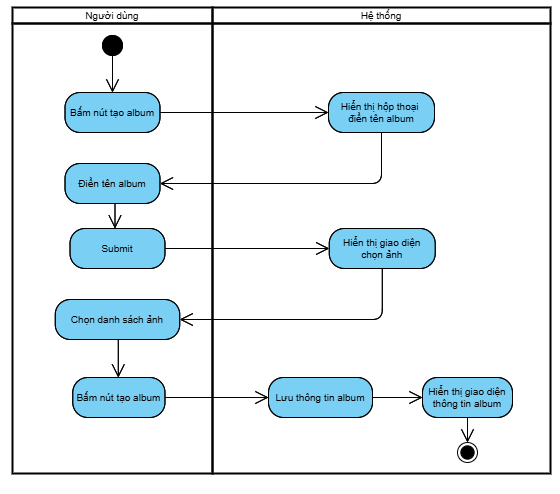
\includegraphics[width=0.6\linewidth]{figures/c3/3-3-7-activity-diagram.png} 
    &  
    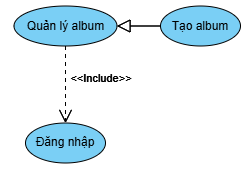
\includegraphics[width=0.35\linewidth]{figures/c3/3-3-7-relationship.png} \\ 
    \hline
\end{tabular}

\begin{figure}[H]
    \centering  
    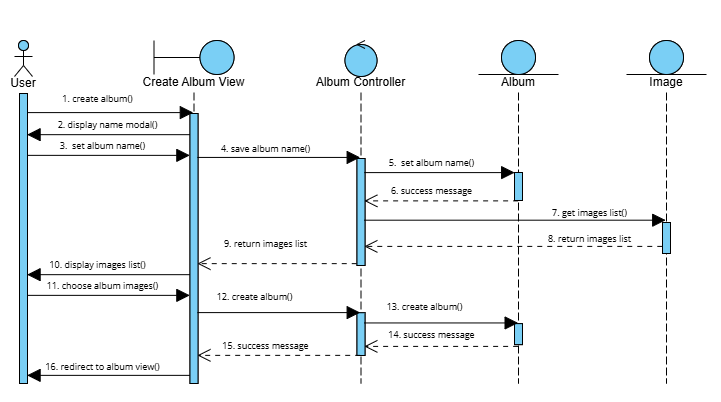
\includegraphics[width=1\textwidth]{figures/c3/3-3-7-sequence-diagram.png}
    \caption{Biểu đồ tuần tự ca sử dụng tạo album.}
    \label{fig:3-3-7-sequence-diagram}
\end{figure}
